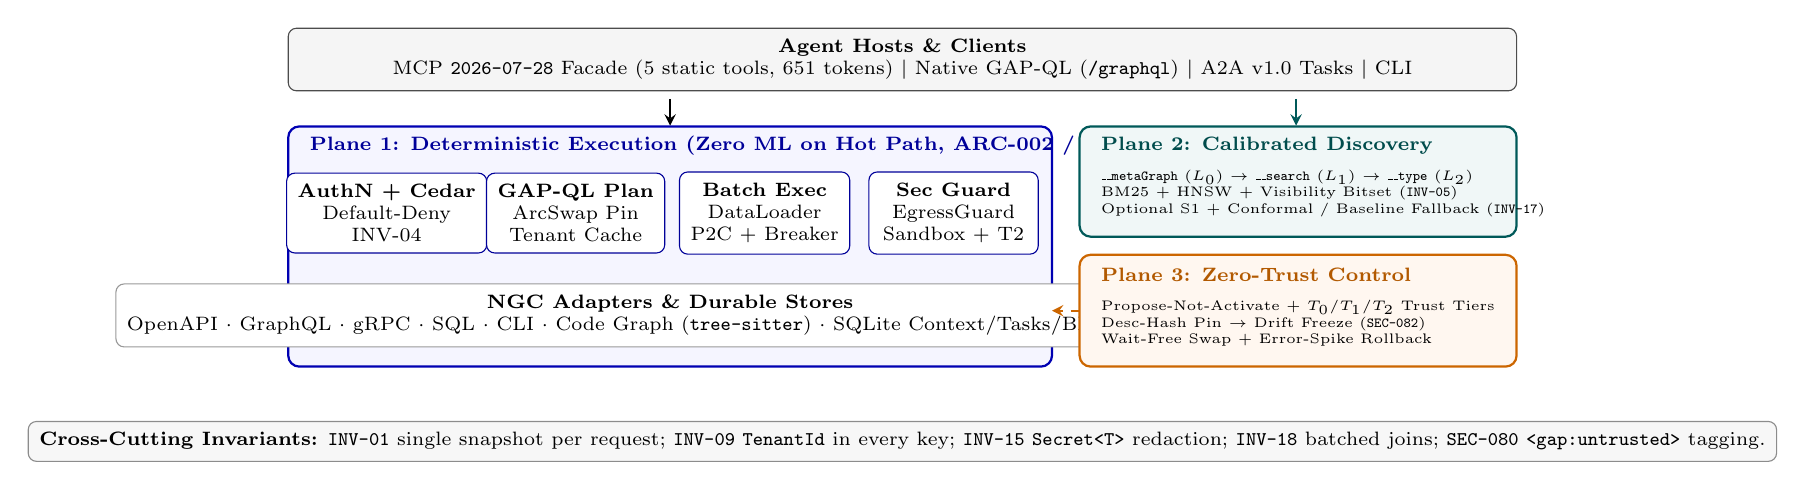
\begin{tikzpicture}[
  box/.style={draw, rounded corners=3pt, align=center, font=\scriptsize, inner sep=4pt, fill=white},
  plane/.style={draw, rounded corners=4pt, thick, inner sep=6pt},
  >=stealth
]
  \node[box, fill=gray!8, minimum width=15.6cm, draw=black!70] (hosts) at (0, 3.6)
    {\textbf{Agent Hosts \& Clients}\\
     MCP \texttt{2026-07-28} Facade (5 static tools, 651 tokens) $\mid$ Native GAP-QL (\texttt{/graphql}) $\mid$ A2A v1.0 Tasks $\mid$ CLI};

  \draw[fill=blue!4, draw=blue!70!black, rounded corners=4pt, thick] (-7.8, -0.3) rectangle (1.9, 2.75);
  \node[anchor=west, font=\scriptsize\bfseries, text=blue!60!black] at (-7.65, 2.50)
    {Plane 1: Deterministic Execution (Zero ML on Hot Path, ARC-002 / INV-01 / INV-02)};

  \node[box, draw=blue!60!black, minimum width=2.15cm, minimum height=0.95cm] (auth) at (-6.55, 1.65)
    {\textbf{AuthN + Cedar}\\Default-Deny\\INV-04};
  \node[box, draw=blue!60!black, minimum width=2.15cm, minimum height=0.95cm] (plan) at (-4.15, 1.65)
    {\textbf{GAP-QL Plan}\\ArcSwap Pin\\Tenant Cache};
  \node[box, draw=blue!60!black, minimum width=2.15cm, minimum height=0.95cm] (exec) at (-1.75, 1.65)
    {\textbf{Batch Exec}\\DataLoader\\P2C + Breaker};
  \node[box, draw=blue!60!black, minimum width=2.15cm, minimum height=0.95cm] (guard) at (0.65, 1.65)
    {\textbf{Sec Guard}\\EgressGuard\\Sandbox + T2};

  \node[box, draw=black!40, minimum width=9.2cm, minimum height=0.8cm] (ngc) at (-2.95, 0.35)
    {\textbf{NGC Adapters \& Durable Stores}\\
     OpenAPI $\cdot$ GraphQL $\cdot$ gRPC $\cdot$ SQL $\cdot$ CLI $\cdot$ Code Graph (\texttt{tree-sitter}) $\cdot$ SQLite Context/Tasks/BLAKE3 Audit};

  \draw[fill=teal!6, draw=teal!70!black, rounded corners=4pt, thick] (2.25, 1.35) rectangle (7.8, 2.75);
  \node[anchor=west, font=\scriptsize\bfseries, text=teal!60!black] at (2.4, 2.50) {Plane 2: Calibrated Discovery};
  \node[anchor=west, font=\tiny, align=left] at (2.4, 1.90)
    {\texttt{\_\_metaGraph} ($L_0$) $\rightarrow$ \texttt{\_\_search} ($L_1$) $\rightarrow$ \texttt{\_\_type} ($L_2$)\\
     BM25 + HNSW + Visibility Bitset (\texttt{INV-05})\\
     Optional S1 + Conformal / Baseline Fallback (\texttt{INV-17})};

  \draw[fill=orange!6, draw=orange!80!black, rounded corners=4pt, thick] (2.25, -0.3) rectangle (7.8, 1.12);
  \node[anchor=west, font=\scriptsize\bfseries, text=orange!70!black] at (2.4, 0.87) {Plane 3: Zero-Trust Control};
  \node[anchor=west, font=\tiny, align=left] at (2.4, 0.25)
    {Propose-Not-Activate + $T_0/T_1/T_2$ Trust Tiers\\
     Desc-Hash Pin $\rightarrow$ Drift Freeze (\texttt{SEC-082})\\
     Wait-Free Swap + Error-Spike Rollback};

  \node[box, fill=gray!6, draw=black!45, minimum width=15.6cm, align=left] (inv) at (0, -1.25)
    {\textbf{Cross-Cutting Invariants:} \texttt{INV-01} single snapshot per request; \texttt{INV-09} \texttt{TenantId} in every key; \texttt{INV-15} \texttt{Secret<T>} redaction; \texttt{INV-18} batched joins; \texttt{SEC-080} \texttt{<gap:untrusted>} tagging.};

  \draw[->, thick] (-2.95, 3.10) -- (-2.95, 2.76);
  \draw[->, thick, draw=teal!70!black] (5.0, 3.10) -- (5.0, 2.76);
  \draw[->, dashed, thick, draw=orange!80!black] (2.25, 0.41) -- (1.90, 0.41);
\end{tikzpicture}

